% THIS IS AN EXAMPLE DOCUMENT FOR VLDB 2012
% based on ACM SIGPROC-SP.TEX VERSION 2.7
% Modified by  Gerald Weber <gerald@cs.auckland.ac.nz>
% Removed the requirement to include *bbl file in here. (AhmetSacan, Sep2012)
% Fixed the equation on page 3 to prevent line overflow. (AhmetSacan, Sep2012)

\documentclass{vldb}
\usepackage{graphicx}
\usepackage{hyperref}
\usepackage{balance}  % for  \balance command ON LAST PAGE  (only there!)


\begin{document}

% ****************** TITLE ****************************************

\title{Global Warming Distributed Data Analysis}

% possible, but not really needed or used for PVLDB:
%\subtitle{[Extended Abstract]
%\titlenote{A full version of this paper is available as\textit{Author's Guide to Preparing ACM SIG Proceedings Using \LaTeX$2_\epsilon$\ and BibTeX} at \texttt{www.acm.org/eaddress.htm}}}

% ****************** AUTHORS **************************************

% You need the command \numberofauthors to handle the 'placement
% and alignment' of the authors beneath the title.
%
% For aesthetic reasons, we recommend 'three authors at a time'
% i.e. three 'name/affiliation blocks' be placed beneath the title.
%
% NOTE: You are NOT restricted in how many 'rows' of
% "name/affiliations" may appear. We just ask that you restrict
% the number of 'columns' to three.
%
% Because of the available 'opening page real-estate'
% we ask you to refrain from putting more than six authors
% (two rows with three columns) beneath the article title.
% More than six makes the first-page appear very cluttered indeed.
%
% Use the \alignauthor commands to handle the names
% and affiliations for an 'aesthetic maximum' of six authors.
% Add names, affiliations, addresses for
% the seventh etc. author(s) as the argument for the
% \additionalauthors command.
% These 'additional authors' will be output/set for you
% without further effort on your part as the last section in
% the body of your article BEFORE References or any Appendices.

\numberofauthors{2} %  in this sample file, there are a *total*
% of EIGHT authors. SIX appear on the 'first-page' (for formatting
% reasons) and the remaining two appear in the \additionalauthors section.

\author{
% You can go ahead and credit any number of authors here,
% e.g. one 'row of three' or two rows (consisting of one row of three
% and a second row of one, two or three).
%
% The command \alignauthor (no curly braces needed) should
% precede each author name, affiliation/snail-mail address and
% e-mail address. Additionally, tag each line of
% affiliation/address with \affaddr, and tag the
% e-mail address with \email.
%
% 1st. author
\alignauthor Alberto Simioni\\
       \affaddr{number}\\
       \email{mail}
% 2nd. author
\alignauthor Federico Ziliotto\\
       \affaddr{2577394}\\
       \email{f.z.ziliotto@student.vu.nl}
}
\date{25 March 2016}


\maketitle

\begin{abstract}


\end{abstract}

\section{Introduction}
Global warming is an open topic of discussion today. While climate scientist debate on the causes of the gradual temperature rise in the past 50 years (the majority claim the increase of CO2 due to fossil fuel is to blame, other researchers found alternative explanations, like non CO2 greenhouse gases (GHGs) \cite{hansen2000global}). Whatever the causes, the data collected by different organizations and from different parts of the world all agree that the global temperature in the world is rising \cite{hansen2006global}. We show that this trend is not only real, but the temperature increase is accelerating in the last twenty years at a worrisome rate. Moreover, we created and interactive tool that may help researchers to visualize the enormous amount of climate data that was collected in the past century and detect possible global warming causes and effects.

\subsection{Data Sources}
We have access to more than one hundred years of weather data provided by the NOAA (National Oceanic and Atmospheric Administration) organization. The raw data is publicly accessible\footnote{\hyperref{ftp://ftp.ncdc.noaa.gov/pub/data/noaa/}} so anyone interested in analyzing the climate of the past years can use them. The data is organized by year and grouped by ISD (Integrated Surface Data) stations. They also provide a \texttt{perl} script that helps in reading and viewing the data. NOAA also publishes monthly reports on the climate status (like temperature, precipitation, sea level) and compares the data obtained for the last month/year to the averages calculated in the past, accompanied by a software suite to repeat or modify the analysis at home. While this tools and datasets are helpful, there are currently no publicly available tools to perform custom data analysis on the whole raw dataset available. In particular, considering the size of the uncompressed data (~200 GB) it may be necessary to use a cluster to make complex computations that require more time. 

\subsection{Our Contribution}
Our aim is to update the recent work done in the climate analysis with the new data available. Moreover, differently than other studies, we will perform the analysis in a cluster and study a way to improve the analysis performance in this type of environment. In the end, we will compare the results we obtained with the ones available in the literature and evaluate the state of global warming in the recent years.\\

In the following sections we first describe the context of our work and the related literature in section \ref{sec:rel}, then we explain how we implemented the data analysis in section \ref{sec:pro}, in section \ref{sec:res} we show the results we obtained and discuss them, and finally in section \ref{sec:con} we argue the relevance of our results and future improvements.


\section{Related Work}
\label{sec:rel}
Studies on global and regional surface temperature change has been done in past. Researchers showed that the rate of temperature increase has been higher in the last quarter of the century that it has been in the previous years of the 20\^{th} century. Moreover they calculated an increase in the average global five year mean of about 1°C\cite{hansen1999giss}. This recent trend is particularly important if we consider the temperature changes in the past millennium, and can be considered an unprecedented anomaly\cite{mann1999northern}. More recent studies also show that the mean annual temperature has not risen in the last twenty years, despite the continuous increase of GHGs in the atmosphere\cite{kosaka2013recent}. This suggests that either the global warming phenomenon that was registered in the period 1975-2000 had different causes or that the more recent stable trend has an origin that balance the greenhouse effects.

\section{Research Question}



\section{Project setup}
\label{sec:pro}
In this section we explain in more detail how we performed the analysis, what tools we used and the preliminary work on the data before the analysis. 


\subsection{Data Format}
The public NOAA data repository contains a file for each station for each year. The name of each file is \{USAF code\}\-\{WBAN code\}-\{year\}, where USAF is the Air Force Station ID and the WBAN is the NCDC (National Climate Data Center) station number. The number of station for each year is shown in figure \ref{fig:stations}. As we can see the number of stations has steadily increased during the years. More importantly, we have to be aware of the results we obtain analyzing years where the number of stations is very low. Since the distribution of the station around the world is not uniform and they don't cover every area, it's difficult to obtain correct results on the global scale. What we can do is to consider the fluctuation of data for the same station or for stations that are near together (this will be done by regional grouping, as described in section \ref{sec:pro}). Each station report data multiple times a day (depending on the station) and for each day of the year.


\begin{figure}[tbh]
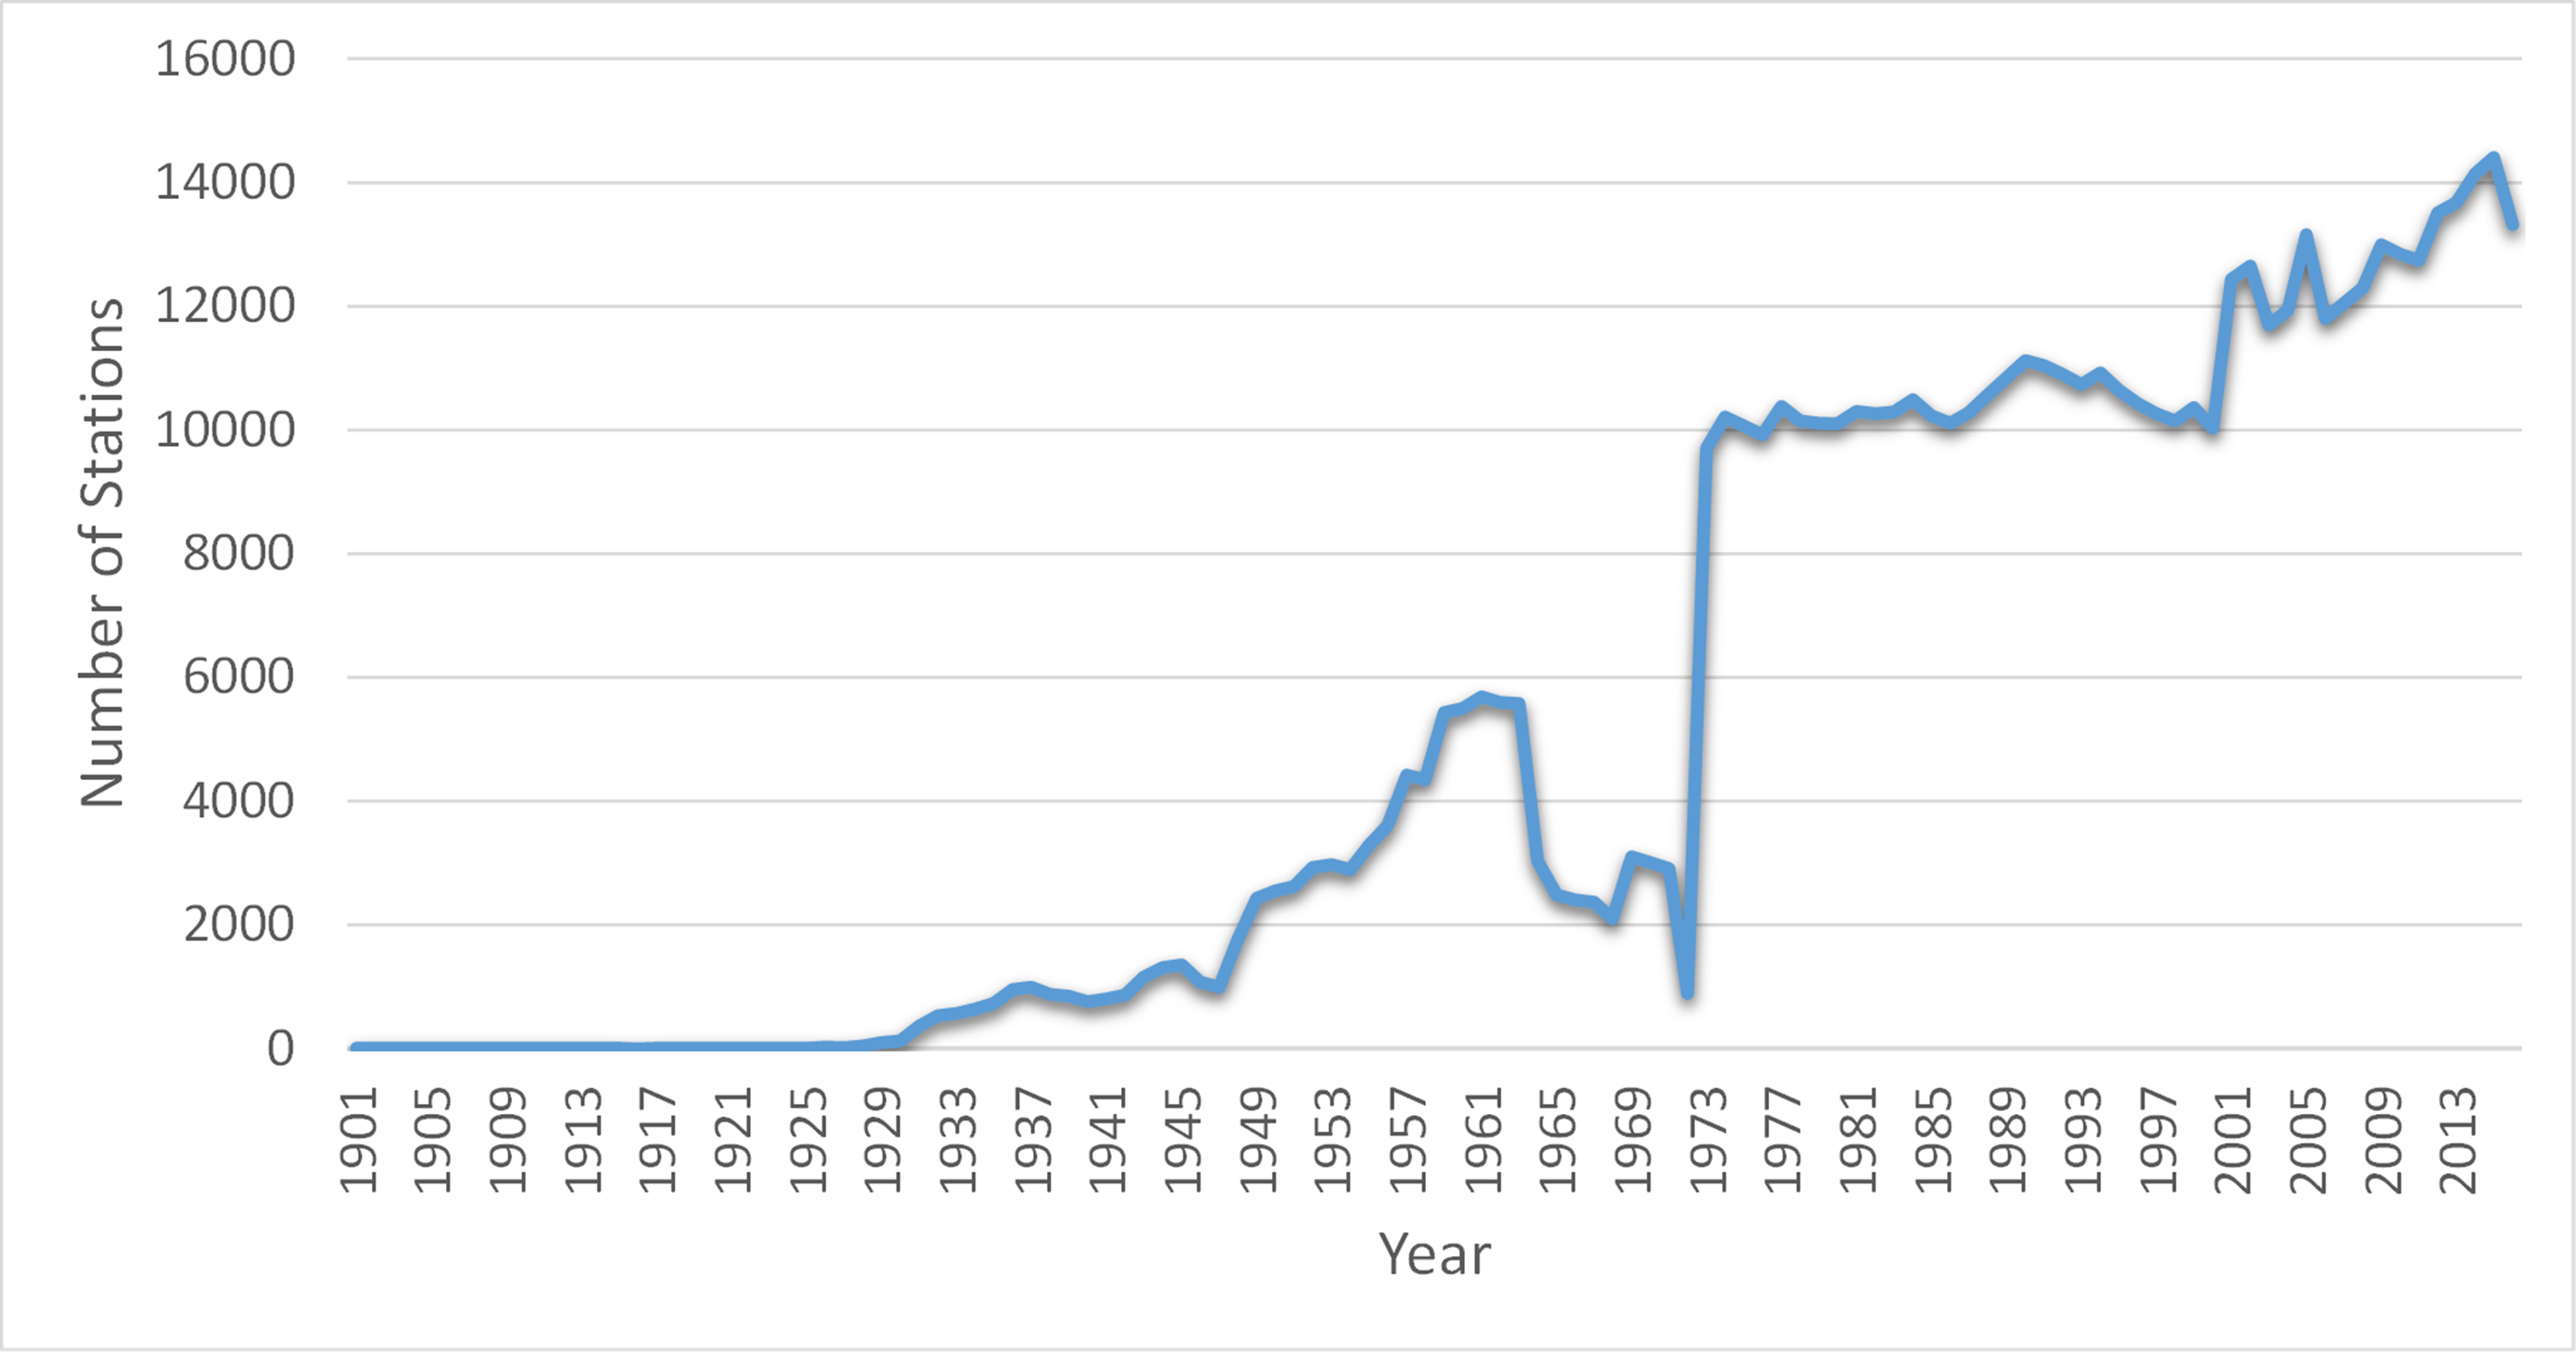
\includegraphics[width=1\linewidth]{stations}
\caption[Stations]{Number of stations per year}
\label{fig:stations}
\end{figure}

noaa data
parser
data filtering, corrupted or erroneous data

\subsection{Distributed environment}
hadoop distributed file system

\subsection{Analysis Tools}
scala

\section{Experiments}
\label{sec:res}


\section{Conclusions}
\label{sec:con}



%\end{document}  % This is where a 'short' article might terminate

% ensure same length columns on last page (might need two sub-sequent latex runs)
\balance

%ACKNOWLEDGMENTS are optional
%\section{Acknowledgments}


% The following two commands are all you need in the
% initial runs of your .tex file to
% produce the bibliography for the citations in your paper.
\bibliographystyle{ieeetr}
\bibliography{vldb_sample}  % vldb_sample.bib is the name of the Bibliography in this case
% You must have a proper ".bib" file
%  and remember to run:
% latex bibtex latex latex
% to resolve all references

%Generated by bibtex from your ~.bib file.  Run latex,
%then bibtex, then latex twice (to resolve references).




\end{document}
